%\documentclass[a4paper,12pt]{report}
\documentclass[a4paper,12pt]{extreport}

\bibliographystyle{iopart-num}
\usepackage{amsmath}
%\usepackage{citesort}
\usepackage{subfigure}
\usepackage{graphicx}
\graphicspath{{fig/}}
\usepackage{ifpdf}
\ifpdf\usepackage{epstopdf}\fi
\usepackage[export]{adjustbox}
\usepackage[numbers]{natbib}

\def\apj{ApJ}
\def\apjl{ApJ Lett.}
\def\mnras{MNRAS}
\def\nat{Nature}
\def\physrevB{Phys. Rev. B}
\def\prd{Phys. Rev. D}
\def\prl{Phys. Rev. Lett.}
\def\pre{Phys. Rev. E}
\def\araa{Ann. Rev. Astron. Astrophys.}                % "Ann. Rev. Astron. Astrophys."
\def\aap{Astron. Astrophys.}                  % "Astron. Astrophys."
\def\aaps{Astron. Astrophys. Suppl. Ser.}                 % "Astron. Astrophys. Suppl. Ser."
\def\aj{Astron. J.}                      % "Astron. J."
\def\apjs{Astrophys. J. Suppl. Ser.}                  % "Astrophys. J. Suppl. Ser."
\def\pasp{Publ. Astron. Soc. Pac.}                  % "Publ. Astron. Soc. Pac."
\def\apjl{ApJ Lett.}                   % letter at ApJ
\def\pasj{PASJ}
\def\apss{Astroph. Space Sci.}
\def\aplett{Astroph. Lett.}
\def\ssr{Space Sci. Rev.}
\def\jcap{J. Cosmol. Astropart. Phys.}
\def\apspr{Sov. Sci. Rev. Sect. E}
\def\nar{New Astron. Rev.}
\def\aapr{ Astron. Astrophys. Rev.}

\begin{document}
	\title{On X-ray emission from Fast Blue Optical Transients}
	
	\author{A M Bykov$^{1}$, V I Romansky$^{1}$}
	

Recent observations of Fast Blue Optical Transients \cite{Margutti2019,Ho2020,Coppejans2020} show high level of X-ray radiation. There are suggested different scenarios of  origins of this radiation: central engine or interaction of shock with external medium. In this paper we present model of interaction of shock with strong wind from close star, producing strong X-ray emission via inverse compton scattering on the photons of this star.

%написать почему не хватает комптона от всей оболочки
\section{hydrodynamic}
In our model we took two close stars, on a distance $1.4\cdot10^{17} cm$, wich correspondes to the radius of expanding shock of CSS161010 at 99 day after explosion. Such small distances are possible in young massive star clusters \cite{}. Also massive star clusters usually have dozens of bright stars with powerfull stellar winds (OB, Wolf-Rayet, and red supergiants). We will refer to them as first star - stable, generating wind, and the second - exploded as supernova. We assumed both stars have winds with velocity $v_w = ?$ and mass loss $\dot{M} = 10^{-5} M_\odot $ per year and luminocity $L=500000 L_\odot$ and surfece temperature $T = 2.5\cdot10^6 K$ which is typical for Wolf-Rayet stars. The magnetic fied of the wind is initialized using \cite{}, and for the first star  it's amplitude is $100 G$ at the radius $10$ while for the second we need much stronger field to satisfy synchrotron observational data, as it is shown in papers \cite{Coppejans2020, BykovUniverse}. So we took magnetic field $1000 G$ at the radius $10^{12}$, stars with such strong fields are described in \cite{}.

For hydrodinamcal simulation we use code PLUTO \cite{MignonePluto}. We used several nested setups on different scales. At first we performed 3d modeling of two stable stars with parameters described above until they winds form a stable configuration. Sizes of the simulation box are $Lx = $ with number of grid points respectively. The next step was 1d spherical modeling of second star explosion. We use ejecta mass $M_{ej} = 0.02 M_\odot$ and velocity $v_{ej} = 0.3 c$ and initial conditions as described in \cite{}. At the third step we use results of the previous steps as initial and boundary conditions in setup with smaller scale - with size $Lx = $ . And at the last step, in setup with the smallest scale $Lx = $, wich is necessary to resolve bow- and tremination shock of the wind of the first star, we use results of the third step as initial and boundary conditions. Scheme of setups is shown in Figure \ref{}.

Simulations showed that ejecta of supernovae, moving in interstellar medium has profile with thin and dense peak, with parameters number density $n \approx 10^5$ and width $d = 1E^{15}$.


The wind shock has radius $R_w \approx 0.5\times10^14 cm$ and number density $n_w \approx 10^9 cm^{-3}$. With this parameters, and luminocity and temperature of the star, one can estimate observed X-ray flux, produxed by inverse compton scattering.

\begin{figure}[h!]
	\centering
	\begin{minipage}{0.48\textwidth}
		\centering
		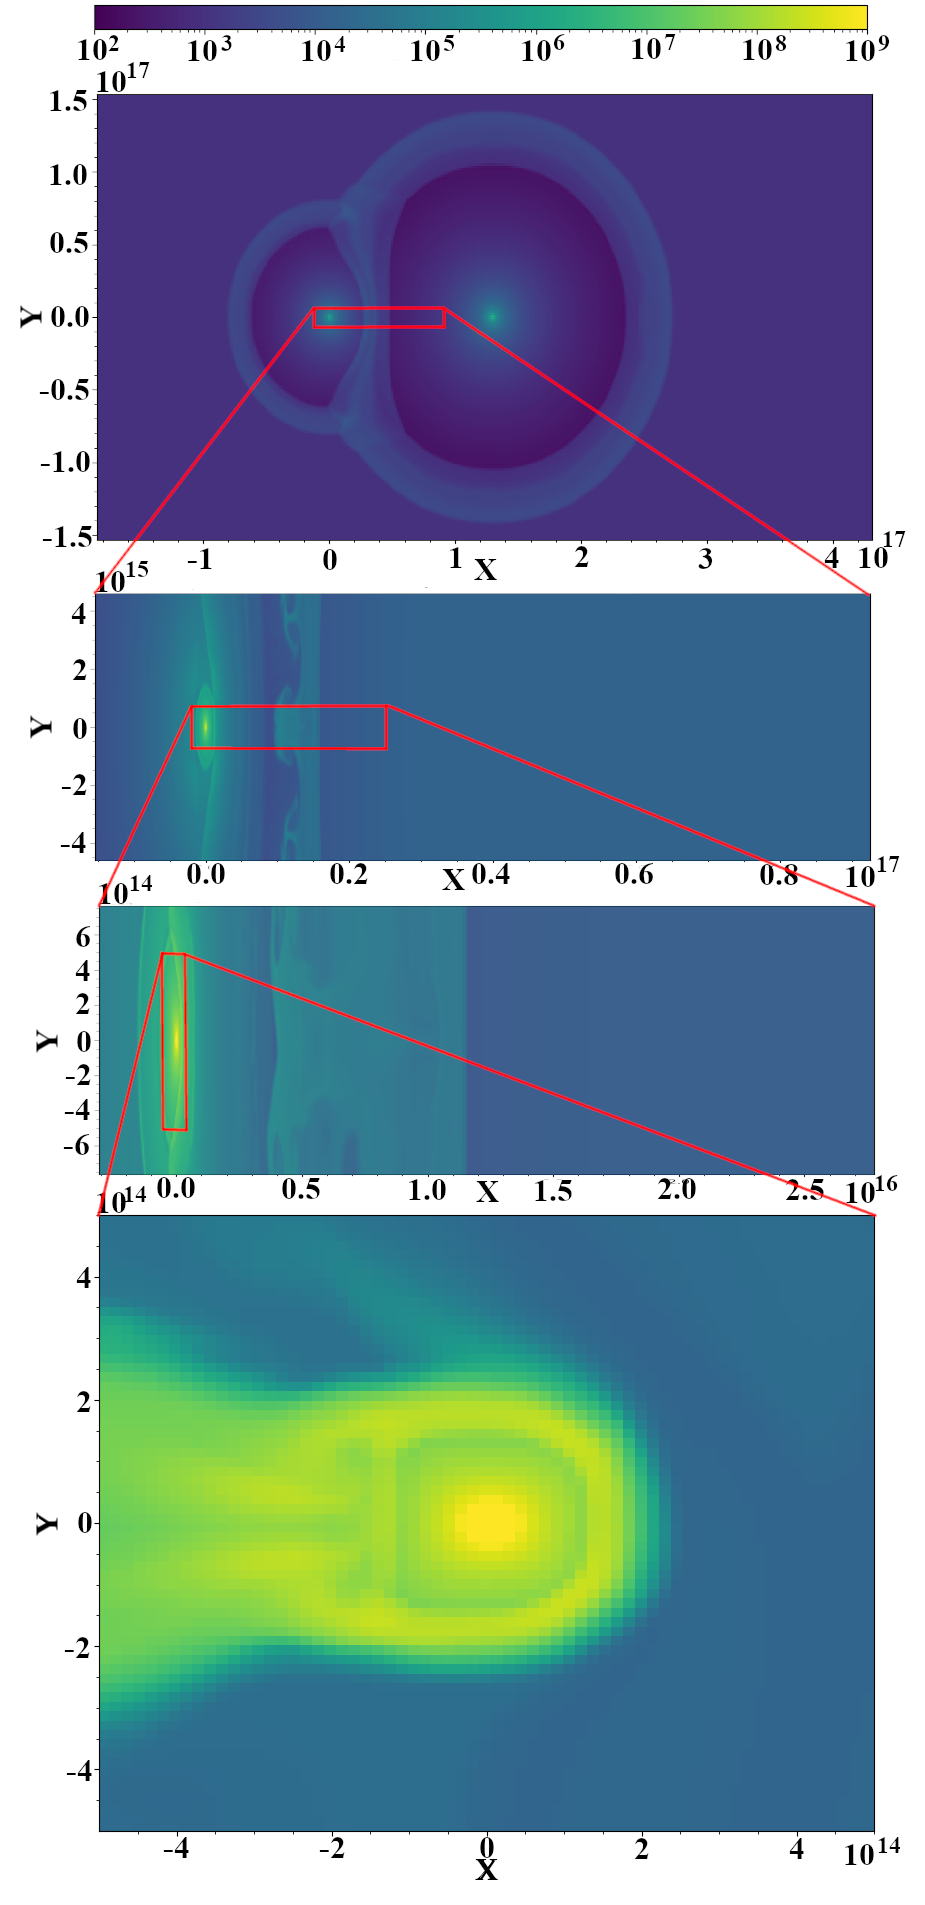
\includegraphics[width=0.98\textwidth]{./fig/density.png} 
		\caption{Density profile of the system at different time moments}
		\label{density}
	\end{minipage}\hfill
	\begin{minipage}{0.48\textwidth}
		\centering
		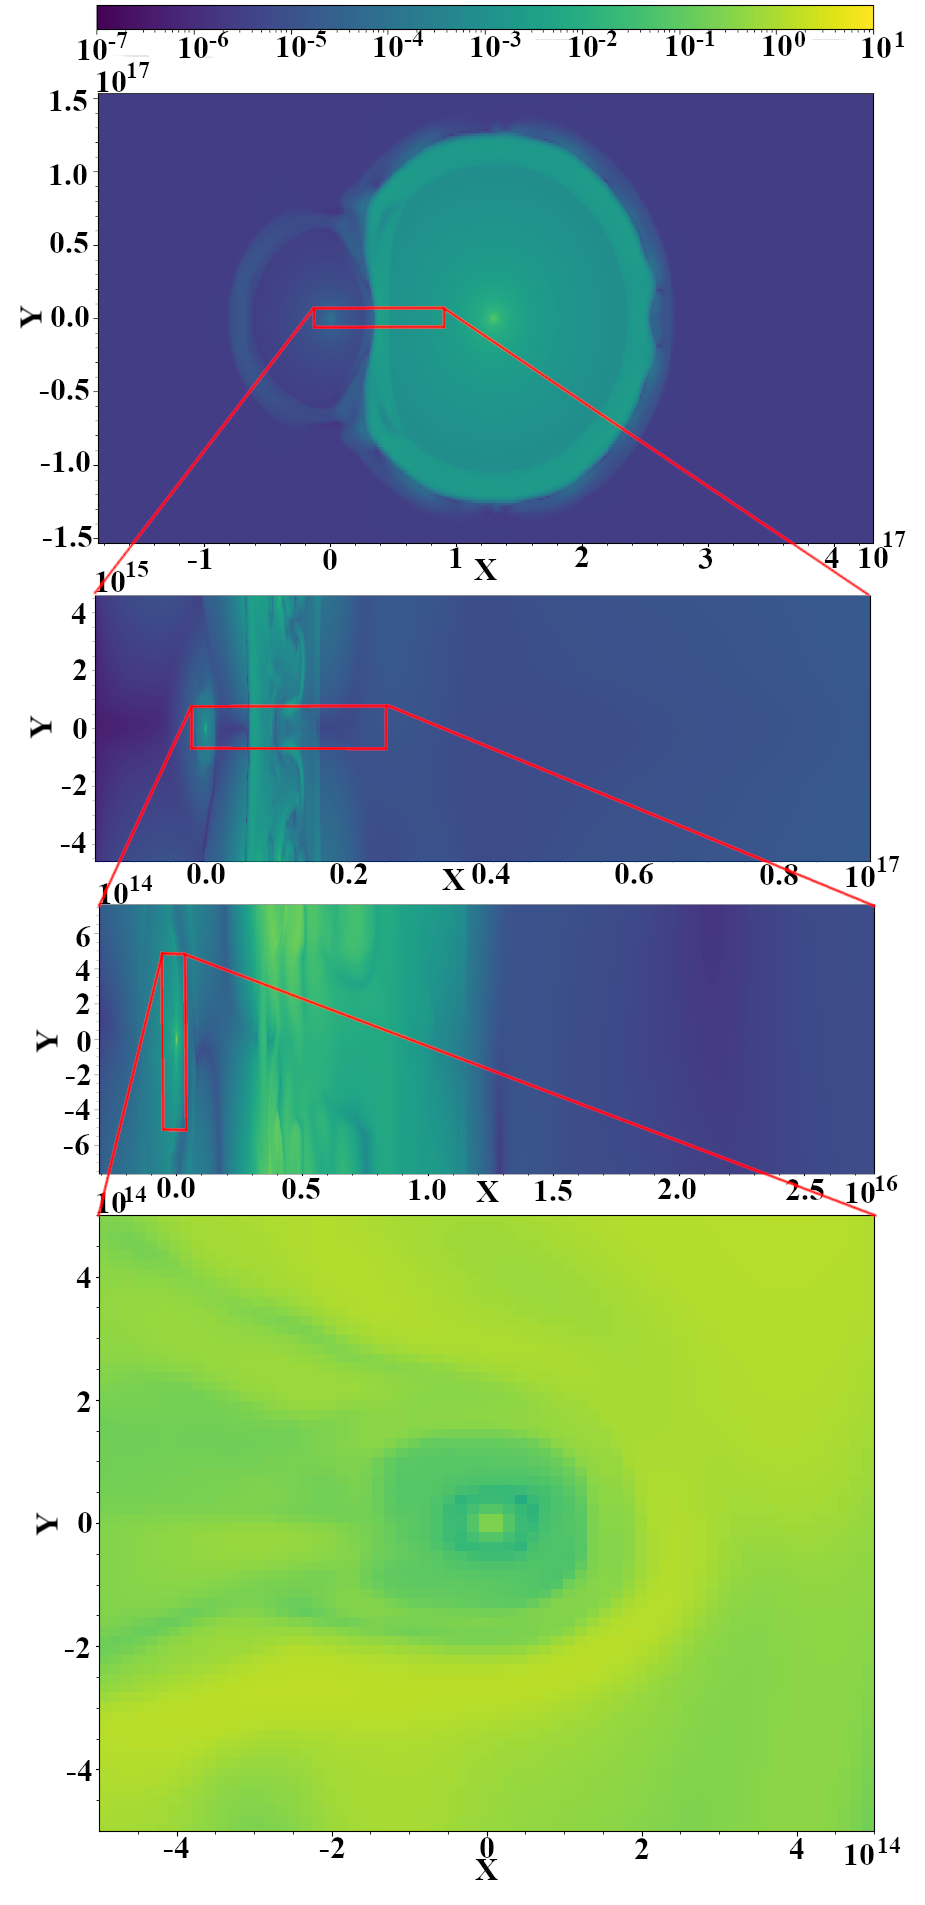
\includegraphics[width=0.98\textwidth]{./fig/Bfield.png} 
		\caption{Magnetic field profile of the system at different time moments}
		\label{Bfield}
	\end{minipage}
\end{figure}
 
\section{radiation}
For evaluating radiation we use our numerical code FAINA, which allows to evaluate synchrotron and inverse compton radiation and also fit model to observational data. 

We assume that source of synchrotron radio flux, observed from CSS161010 is spherical shell with uniform density and magnetic field. Distribution function of emitting is evaluated using PIC simulation with code SMILEI \cite{Derouillat}. Setups for shock simulation is decribed in details in our previous work \cite{BykovUniverse}. Shock was initialized due to collision of uniform plasma flow with velocity $0.3 c$ with reflecting wall. Magnetiztion was $\sigma = B^2/4 pi m_p \gamma c^2 = 0.002$ and diffirent inclination angles of magnetic field were studied. Distributions for different inclination angles of magnetic field relative to local shock velocity are taken in different points of the source. With this assumptions we can fit our model to observational data of radio flux from CSS161010 at 98 day after explosion (the first observation when both radio and X-ray flux was detected), and derive such parameters as magnetic field, concentration and width of the spherical shell. Our best fit for radio flux and observational data are shown on Figure \ref{}. Evaluated parameters are magnetic field $B = 0.6 G$, number density $n = 50000{cm}^{-3}$ and shell width $l = 0.01\cdot R = 1.3E15 cm$. This parameters are consistent with obtained from hydrodynamical simulations.

In our model X-ray flux is generated via inverse compton scattering in the region of iteraction between wind from the first star, and supernova ejecta from the second. Relativistic ejecta has huge bulk pressure and wind is compressed to small region with high number dencity. Also this region is close to high luminous star, and there are suitable conditions for strong inverse compton radiation. Electrons can be accelerated on the shock fronts or on the shearing flows. So electrons distribution function is 
%непонятно чт писать
We assume that source is a cylinder with radius $R_w$, and height also equals $R_w$, with axis oriendted along line of sight, and with uniform number density $n_w$. 
and photons distribution corresponds to the radiation of the first star at distance $R_w$. With this parameter modeled X-ray flux in the energy range $0.3-10 keV$ is $F_m = $ which is consistent with observed flux of CSS161010 at 99 day after explosion $F_{obs = }$ \cite{Coppejans2020}.

\bibliographystyle{iopart-num}
\bibliography{fbotcompton}
\end{document}